%% bare_conf_compsoc.tex
%% V1.4b
%% 2015/08/26
%% by Michael Shell
%% See:
%% http://www.michaelshell.org/
%% for current contact information.
%%
%% This is a skeleton file demonstrating the use of IEEEtran.cls
%% (requires IEEEtran.cls version 1.8b or later) with an IEEE Computer
%% Society conference paper.
%%
%% Support sites:
%% http://www.michaelshell.org/tex/ieeetran/
%% http://www.ctan.org/pkg/ieeetran
%% and
%% http://www.ieee.org/

%%*************************************************************************
%% Legal Notice:
%% This code is offered as-is without any warranty either expressed or
%% implied; without even the implied warranty of MERCHANTABILITY or
%% FITNESS FOR A PARTICULAR PURPOSE! 
%% User assumes all risk.
%% In no event shall the IEEE or any contributor to this code be liable for
%% any damages or losses, including, but not limited to, incidental,
%% consequential, or any other damages, resulting from the use or misuse
%% of any information contained here.
%%
%% All comments are the opinions of their respective authors and are not
%% necessarily endorsed by the IEEE.
%%
%% This work is distributed under the LaTeX Project Public License (LPPL)
%% ( http://www.latex-project.org/ ) version 1.3, and may be freely used,
%% distributed and modified. A copy of the LPPL, version 1.3, is included
%% in the base LaTeX documentation of all distributions of LaTeX released
%% 2003/12/01 or later.
%% Retain all contribution notices and credits.
%% ** Modified files should be clearly indicated as such, including  **
%% ** renaming them and changing author support contact information. **
%%*************************************************************************


% *** Authors should verify (and, if needed, correct) their LaTeX system  ***
% *** with the testflow diagnostic prior to trusting their LaTeX platform ***
% *** with production work. The IEEE's font choices and paper sizes can   ***
% *** trigger bugs that do not appear when using other class files.       ***                          ***
% The testflow support page is at:
% http://www.michaelshell.org/tex/testflow/



\documentclass[conference,compsoc]{IEEEtran}
% Some/most Computer Society conferences require the compsoc mode option,
% but others may want the standard conference format.
%
% If IEEEtran.cls has not been installed into the LaTeX system files,
% manually specify the path to it like:
% \documentclass[conference,compsoc]{../sty/IEEEtran}





% Some very useful LaTeX packages include:
% (uncomment the ones you want to load)


% *** MISC UTILITY PACKAGES ***
%
%\usepackage{ifpdf}
% Heiko Oberdiek's ifpdf.sty is very useful if you need conditional
% compilation based on whether the output is pdf or dvi.
% usage:
% \ifpdf
%   % pdf code
% \else
%   % dvi code
% \fi
% The latest version of ifpdf.sty can be obtained from:
% http://www.ctan.org/pkg/ifpdf
% Also, note that IEEEtran.cls V1.7 and later provides a builtin
% \ifCLASSINFOpdf conditional that works the same way.
% When switching from latex to pdflatex and vice-versa, the compiler may
% have to be run twice to clear warning/error messages.






% *** CITATION PACKAGES ***
%
\ifCLASSOPTIONcompsoc
  % IEEE Computer Society needs nocompress option
  % requires cite.sty v4.0 or later (November 2003)
  \usepackage[nocompress]{cite}
\else
  % normal IEEE
  \usepackage{cite}
\fi
% cite.sty was written by Donald Arseneau
% V1.6 and later of IEEEtran pre-defines the format of the cite.sty package
% \cite{} output to follow that of the IEEE. Loading the cite package will
% result in citation numbers being automatically sorted and properly
% "compressed/ranged". e.g., [1], [9], [2], [7], [5], [6] without using
% cite.sty will become [1], [2], [5]--[7], [9] using cite.sty. cite.sty's
% \cite will automatically add leading space, if needed. Use cite.sty's
% noadjust option (cite.sty V3.8 and later) if you want to turn this off
% such as if a citation ever needs to be enclosed in parenthesis.
% cite.sty is already installed on most LaTeX systems. Be sure and use
% version 5.0 (2009-03-20) and later if using hyperref.sty.
% The latest version can be obtained at:
% http://www.ctan.org/pkg/cite
% The documentation is contained in the cite.sty file itself.
%
% Note that some packages require special options to format as the Computer
% Society requires. In particular, Computer Society  papers do not use
% compressed citation ranges as is done in typical IEEE papers
% (e.g., [1]-[4]). Instead, they list every citation separately in order
% (e.g., [1], [2], [3], [4]). To get the latter we need to load the cite
% package with the nocompress option which is supported by cite.sty v4.0
% and later.





% *** GRAPHICS RELATED PACKAGES ***
%
\ifCLASSINFOpdf
  \usepackage[pdftex]{graphicx}
  % declare the path(s) where your graphic files are
  % \graphicspath{{../pdf/}{../jpeg/}}
  % and their extensions so you won't have to specify these with
  % every instance of \includegraphics
  % \DeclareGraphicsExtensions{.pdf,.jpeg,.png}
\else
  % or other class option (dvipsone, dvipdf, if not using dvips). graphicx
  % will default to the driver specified in the system graphics.cfg if no
  % driver is specified.
  % \usepackage[dvips]{graphicx}
  % declare the path(s) where your graphic files are
  % \graphicspath{{../eps/}}
  % and their extensions so you won't have to specify these with
  % every instance of \includegraphics
  % \DeclareGraphicsExtensions{.eps}
\fi
% graphicx was written by David Carlisle and Sebastian Rahtz. It is
% required if you want graphics, photos, etc. graphicx.sty is already
% installed on most LaTeX systems. The latest version and documentation
% can be obtained at: 
% http://www.ctan.org/pkg/graphicx
% Another good source of documentation is "Using Imported Graphics in
% LaTeX2e" by Keith Reckdahl which can be found at:
% http://www.ctan.org/pkg/epslatex
%
% latex, and pdflatex in dvi mode, support graphics in encapsulated
% postscript (.eps) format. pdflatex in pdf mode supports graphics
% in .pdf, .jpeg, .png and .mps (metapost) formats. Users should ensure
% that all non-photo figures use a vector format (.eps, .pdf, .mps) and
% not a bitmapped formats (.jpeg, .png). The IEEE frowns on bitmapped formats
% which can result in "jaggedy"/blurry rendering of lines and letters as
% well as large increases in file sizes.
%
% You can find documentation about the pdfTeX application at:
% http://www.tug.org/applications/pdftex





% *** MATH PACKAGES ***
%
%\usepackage{amsmath}
% A popular package from the American Mathematical Society that provides
% many useful and powerful commands for dealing with mathematics.
%
% Note that the amsmath package sets \interdisplaylinepenalty to 10000
% thus preventing page breaks from occurring within multiline equations. Use:
%\interdisplaylinepenalty=2500
% after loading amsmath to restore such page breaks as IEEEtran.cls normally
% does. amsmath.sty is already installed on most LaTeX systems. The latest
% version and documentation can be obtained at:
% http://www.ctan.org/pkg/amsmath





% *** SPECIALIZED LIST PACKAGES ***
%
%\usepackage{algorithmic}
% algorithmic.sty was written by Peter Williams and Rogerio Brito.
% This package provides an algorithmic environment fo describing algorithms.
% You can use the algorithmic environment in-text or within a figure
% environment to provide for a floating algorithm. Do NOT use the algorithm
% floating environment provided by algorithm.sty (by the same authors) or
% algorithm2e.sty (by Christophe Fiorio) as the IEEE does not use dedicated
% algorithm float types and packages that provide these will not provide
% correct IEEE style captions. The latest version and documentation of
% algorithmic.sty can be obtained at:
% http://www.ctan.org/pkg/algorithms
% Also of interest may be the (relatively newer and more customizable)
% algorithmicx.sty package by Szasz Janos:
% http://www.ctan.org/pkg/algorithmicx




% *** ALIGNMENT PACKAGES ***
%
%\usepackage{array}
% Frank Mittelbach's and David Carlisle's array.sty patches and improves
% the standard LaTeX2e array and tabular environments to provide better
% appearance and additional user controls. As the default LaTeX2e table
% generation code is lacking to the point of almost being broken with
% respect to the quality of the end results, all users are strongly
% advised to use an enhanced (at the very least that provided by array.sty)
% set of table tools. array.sty is already installed on most systems. The
% latest version and documentation can be obtained at:
% http://www.ctan.org/pkg/array


% IEEEtran contains the IEEEeqnarray family of commands that can be used to
% generate multiline equations as well as matrices, tables, etc., of high
% quality.




% *** SUBFIGURE PACKAGES ***
%\ifCLASSOPTIONcompsoc
%  \usepackage[caption=false,font=footnotesize,labelfont=sf,textfont=sf]{subfig}
%\else
%  \usepackage[caption=false,font=footnotesize]{subfig}
%\fi
% subfig.sty, written by Steven Douglas Cochran, is the modern replacement
% for subfigure.sty, the latter of which is no longer maintained and is
% incompatible with some LaTeX packages including fixltx2e. However,
% subfig.sty requires and automatically loads Axel Sommerfeldt's caption.sty
% which will override IEEEtran.cls' handling of captions and this will result
% in non-IEEE style figure/table captions. To prevent this problem, be sure
% and invoke subfig.sty's "caption=false" package option (available since
% subfig.sty version 1.3, 2005/06/28) as this is will preserve IEEEtran.cls
% handling of captions.
% Note that the Computer Society format requires a sans serif font rather
% than the serif font used in traditional IEEE formatting and thus the need
% to invoke different subfig.sty package options depending on whether
% compsoc mode has been enabled.
%
% The latest version and documentation of subfig.sty can be obtained at:
% http://www.ctan.org/pkg/subfig




% *** FLOAT PACKAGES ***
%
%\usepackage{fixltx2e}
% fixltx2e, the successor to the earlier fix2col.sty, was written by
% Frank Mittelbach and David Carlisle. This package corrects a few problems
% in the LaTeX2e kernel, the most notable of which is that in current
% LaTeX2e releases, the ordering of single and double column floats is not
% guaranteed to be preserved. Thus, an unpatched LaTeX2e can allow a
% single column figure to be placed prior to an earlier double column
% figure.
% Be aware that LaTeX2e kernels dated 2015 and later have fixltx2e.sty's
% corrections already built into the system in which case a warning will
% be issued if an attempt is made to load fixltx2e.sty as it is no longer
% needed.
% The latest version and documentation can be found at:
% http://www.ctan.org/pkg/fixltx2e


%\usepackage{stfloats}
% stfloats.sty was written by Sigitas Tolusis. This package gives LaTeX2e
% the ability to do double column floats at the bottom of the page as well
% as the top. (e.g., "\begin{figure*}[!b]" is not normally possible in
% LaTeX2e). It also provides a command:
%\fnbelowfloat
% to enable the placement of footnotes below bottom floats (the standard
% LaTeX2e kernel puts them above bottom floats). This is an invasive package
% which rewrites many portions of the LaTeX2e float routines. It may not work
% with other packages that modify the LaTeX2e float routines. The latest
% version and documentation can be obtained at:
% http://www.ctan.org/pkg/stfloats
% Do not use the stfloats baselinefloat ability as the IEEE does not allow
% \baselineskip to stretch. Authors submitting work to the IEEE should note
% that the IEEE rarely uses double column equations and that authors should try
% to avoid such use. Do not be tempted to use the cuted.sty or midfloat.sty
% packages (also by Sigitas Tolusis) as the IEEE does not format its papers in
% such ways.
% Do not attempt to use stfloats with fixltx2e as they are incompatible.
% Instead, use Morten Hogholm'a dblfloatfix which combines the features
% of both fixltx2e and stfloats:
%
% \usepackage{dblfloatfix}
% The latest version can be found at:
% http://www.ctan.org/pkg/dblfloatfix




% *** PDF, URL AND HYPERLINK PACKAGES ***
%
%\usepackage{url}
% url.sty was written by Donald Arseneau. It provides better support for
% handling and breaking URLs. url.sty is already installed on most LaTeX
% systems. The latest version and documentation can be obtained at:
% http://www.ctan.org/pkg/url
% Basically, \url{my_url_here}.




% *** Do not adjust lengths that control margins, column widths, etc. ***
% *** Do not use packages that alter fonts (such as pslatex).         ***
% There should be no need to do such things with IEEEtran.cls V1.6 and later.
% (Unless specifically asked to do so by the journal or conference you plan
% to submit to, of course. )



% \usepackage{background}
% \backgroundsetup{
%   scale=2,
%   color=red,
%   opacity=1,
%   angle=0,
%   vshift=0.5cm,
%   position=current page.south,
%   contents={Confidential and Proprietary - Do not redistribute }
% }


% correct bad hyphenation here
\hyphenation{op-tical net-works semi-conduc-tor}


\begin{document}
%
% paper title
% Titles are generally capitalized except for words such as a, an, and, as,
% at, but, by, for, in, nor, of, on, or, the, to and up, which are usually
% not capitalized unless they are the first or last word of the title.
% Linebreaks \\ can be used within to get better formatting as desired.
% Do not put math or special symbols in the title.
\title{Decentralized AI: Permissionless LLM Inference on POKT Network}


% author names and affiliations
% use a multiple column layout for up to three different
% affiliations
\author{\IEEEauthorblockN{Daniel Olshansky}
\IEEEauthorblockA{Grove Inc.}
\and
\IEEEauthorblockN{Ramiro Rodr\'iguez Colmeiro}
\IEEEauthorblockA{Pocket Scan Technologies LLC}
\and
\IEEEauthorblockN{Bowen Li}
\IEEEauthorblockA{POKT Network Foundation}}

% conference papers do not typically use \thanks and this command
% is locked out in conference mode. If really needed, such as for
% the acknowledgment of grants, issue a \IEEEoverridecommandlockouts
% after \documentclass

% for over three affiliations, or if they all won't fit within the width
% of the page (and note that there is less available width in this regard for
% compsoc conferences compared to traditional conferences), use this
% alternative format:
% 
%\author{\IEEEauthorblockN{Michael Shell\IEEEauthorrefmark{1},
%Homer Simpson\IEEEauthorrefmark{2},
%James Kirk\IEEEauthorrefmark{3}, 
%Montgomery Scott\IEEEauthorrefmark{3} and
%Eldon Tyrell\IEEEauthorrefmark{4}}
%\IEEEauthorblockA{\IEEEauthorrefmark{1}School of Electrical and Computer Engineering\\
%Georgia Institute of Technology,
%Atlanta, Georgia 30332--0250\\ Email: see http://www.michaelshell.org/contact.html}
%\IEEEauthorblockA{\IEEEauthorrefmark{2}Twentieth Century Fox, Springfield, USA\\
%Email: homer@thesimpsons.com}
%\IEEEauthorblockA{\IEEEauthorrefmark{3}Starfleet Academy, San Francisco, California 96678-2391\\
%Telephone: (800) 555--1212, Fax: (888) 555--1212}
%\IEEEauthorblockA{\IEEEauthorrefmark{4}Tyrell Inc., 123 Replicant Street, Los Angeles, California 90210--4321}}




% use for special paper notices
%\IEEEspecialpapernotice{(Invited Paper)}




% make the title area
\maketitle

% As a general rule, do not put math, special symbols or citations
% in the abstract
\begin{abstract}
POKT Network's decentralized Remote Procedure Call (RPC) infrastructure, surpassing 740 billion requests since launching on MainNet in 2020, is well-positioned to extend into providing AI inference services with minimal design or implementation modifications. This litepaper illustrates how the network's open-source and permissionless design aligns incentives among model researchers, hardware operators, API providers and users whom we term model Sources, Suppliers, Gateways and Applications respectively. Through its Relay Mining algorithm, POKT creates a transparent marketplace where costs and earnings directly reflect cryptographically verified usage. This decentralized framework offers large model AI researchers a new avenue to disseminate their work and generate revenue without the complexities of maintaining infrastructure or building end-user products. Supply scales naturally with demand, as evidenced in recent years and the protocol's free market dynamics. POKT Gateways facilitate network growth, evolution, adoption, and quality by acting as application-facing load balancers, providing value-added features without managing LLM nodes directly. This vertically decoupled network, battle tested over several years, is set up to accelerate the adoption, operation, innovation and financialization of open-source models. It is the first mature permissionless network whose quality of service competes with centralized entities set up to provide application grade inference.
\end{abstract}

% no keywords




% For peer review papers, you can put extra information on the cover
% page as needed:
% \ifCLASSOPTIONpeerreview
% \begin{center} \bfseries EDICS Category: 3-BBND \end{center}
% \fi
%
% For peerreview papers, this IEEEtran command inserts a page break and
% creates the second title. It will be ignored for other modes.
\IEEEpeerreviewmaketitle



\section{Introduction}

\subsection{ LLM Inference \& Web3 Full Nodes}
The advent of OpenAI’s ChatGPT brought foundation models into the mainstream. With it, the ecosystem of fine-tuning, distributing, evaluating and optimizing models has become ubiquitous. Companies like Meta are training and open-sourcing~\cite{metaIntroducingMeta} models ranging from 8B (small) to over 400B (large) parameters, often referred to as Language Models (LMs), Large Language Models (LLMs), or Large Multimodal Models (LMMs). Platforms like HuggingFace have become central hubs for sharing and discovering new models, hosting hundreds of thousands~\cite{greataipromptsEveryHugging} of open-source models from institutions and independent researchers.

Although some models can be hosted on personal devices~\cite{pytorchExecuTorchAlpha}, most AI engineers~\cite{latentRiseEngineer} rely on third-party services with less resource-constrained hardware for reliable and cost-effective inference maintained by dedicated teams. These LLM API Providers~\cite{artificialanalysisProviderLeaderboard} create a disjoint and inconsistent ecosystem that varies in models offered, APIs, tooling with little visibility into what drives their cost structure or how new models are added to their offering list.

Delegating infrastructure maintenance to third parties has been common practice in Web3 for years. As the resource requirements for maintaining Full Nodes~\cite{bitcoinRunningFull} increased – Solana~\cite{solanalabsSolanaValidator} recommending a minimum of 512GB of RAM for baseline functionality – the industry began relying on outsourced Remote Procedure Call (RPC) Nodes maintained by full-time DevOps teams. Today, there are dozens of major RPC providers~\cite{rpclistRPCListFind}, each servicing multiple blockchains.

\subsection{POKT Network Background}

POKT Network~\cite{poktWeb3Infrastructure} has been live on MainNet since 2020, serving hundreds of millions of daily RPC requests~\cite{poktscan} across dozens of blockchains via a heterogeneous and independent set of hardware operators. As a Decentralized Physical Infrastructure Network (DePIN), its permissionless and incentive-driven economics drive the organic addition and weeding out of supported blockchains based on customer demand and usage.

The POKT Network protocol's core Relay Mining~\cite{olshansky2023relay} algorithm acts as an on-chain metering system that cryptographically verifies how many network requests were serviced for some Application by a particular Supplier for a given service. Similar to how Bitcoin~\cite{nakamoto2008bitcoin} operates as a permissionless timestamp server, POKT serves as a permissionless, verifiable request counter or optimistic multi-tenant rate limiter. This forces Suppliers to generate a useful proof of work when servicing RPC requests, and incentivizes them to upkeep high-quality, honest services, since Applications will seek alternative providers if quality or honesty declines.

POKT Network provides this via an open internet infrastructure layer which coordinates an established network of Suppliers, atop of which a growing ecosystem of Gateways provide additional products and services. Though Applications can access the network directly, Gateways provide a mechanism to access the protocol's network while abstracting out its complexities. By vertically decoupling in this way, each network participant optimizes an aspect of performance, while preserving open access to infrastructure that is rapidly becoming a core digital public utility. 

\section{Core Problem}

\subsection{The Infrastructure Gaps}

The AI landscape is evolving rapidly and the next few years will be pivotal in determining the balance of open vs closed source foundation models, their financialization, and the API providers that facilitate access to them. Growth, adoption, and returns will be driven by tooling, incentivization and accessibility that creates equal opportunity for all of the stakeholders involved by vertically decoupling the stack and tackling the following challenges:
\begin{itemize}
    \item \textbf{Restricted model experimentation:} the resource-intensive nature of infrastructure restricts the ability of AI researchers and AI-enabled applications to explore a variety of models. Outsourcing that infrastructure to a vertically integrated partner - LLM API Providers - removes the infrastructure constraint but restricts the available range to their supported models. 
    \item \textbf{Lack of a sustainable business model for open source innovation:} independent ML engineers struggle to distribute and monetize their models and are increasingly reliant on being picked up by major infrastructure providers who, in turn, are able to squeeze their incentives. This is not conducive to sustained innovation and the emergence of supportive ecosystems.
    \item \textbf{Unequal market access:} vertically integrated infrastructure companies are incentivized to prioritize enterprise-grade customers who favour top-tier models on high-end hardware. Affordable inference for mid-tier models on mid-tier hardware, therefore, becomes harder to come by, squeezing out the middle of the market.
\end{itemize}

\subsection{POKT Network’s Unique Value Proposition}

POKT Network’s universal RPC infrastructure is perfectly primed to extend to AI Inference of in which:
An application calls a remote server, where the request acts as the prompt.
The remote server runs a procedure (the model).
The Remote Procedure Call (RPC) is completed when the generated response returns to the application.

By vertically decoupling the infrastructure layer from the product and services layer, POKT Network’s foundational infrastructure remains open and fully decentralized, while end users benefit from a growing ecosystem of Gateways that provide competitive levels of innovation, UX, and quality of service. In addition, its on-chain cryptographic rate-limiting design incentivizes high-quality service delivery and creates alignment among all network stakeholders. 

POKT Network enables Decentralized AI Inference through:
\begin{itemize}
    \item \textbf{Proven, Established Network:} Capitalizing on an established network of Suppliers that streamline access to models, along with Gateways that ensure a sufficient quality of service for end users.
    \item \textbf{Separation of Concerns:} Delineating responsibilities across the stack such that each stakeholder only focuses on their strengths to improve the efficiency of the overall ecosystem.
    \item \textbf{Incentive Alignment:} Explicit cryptographic proofs and implicit performance measurements create economic incentive alignment in a vertically decoupled ecosystem that encourages transparent competition.
    \item \textbf{Permissionless Models \& Supply:} As shown by the network’s history, its permissionless nature creates an open data and service marketplace that aggregates cost-effective hardware supply.
\end{itemize}


\section{Decentralized AI Inference Stakeholders}

A comparison of the decentralized stack versus the centralized providers is shown in figure~\ref{fig_stakeholders}. Each participant is described below (from top to bottom):

\begin{figure*}[!h]
\centering
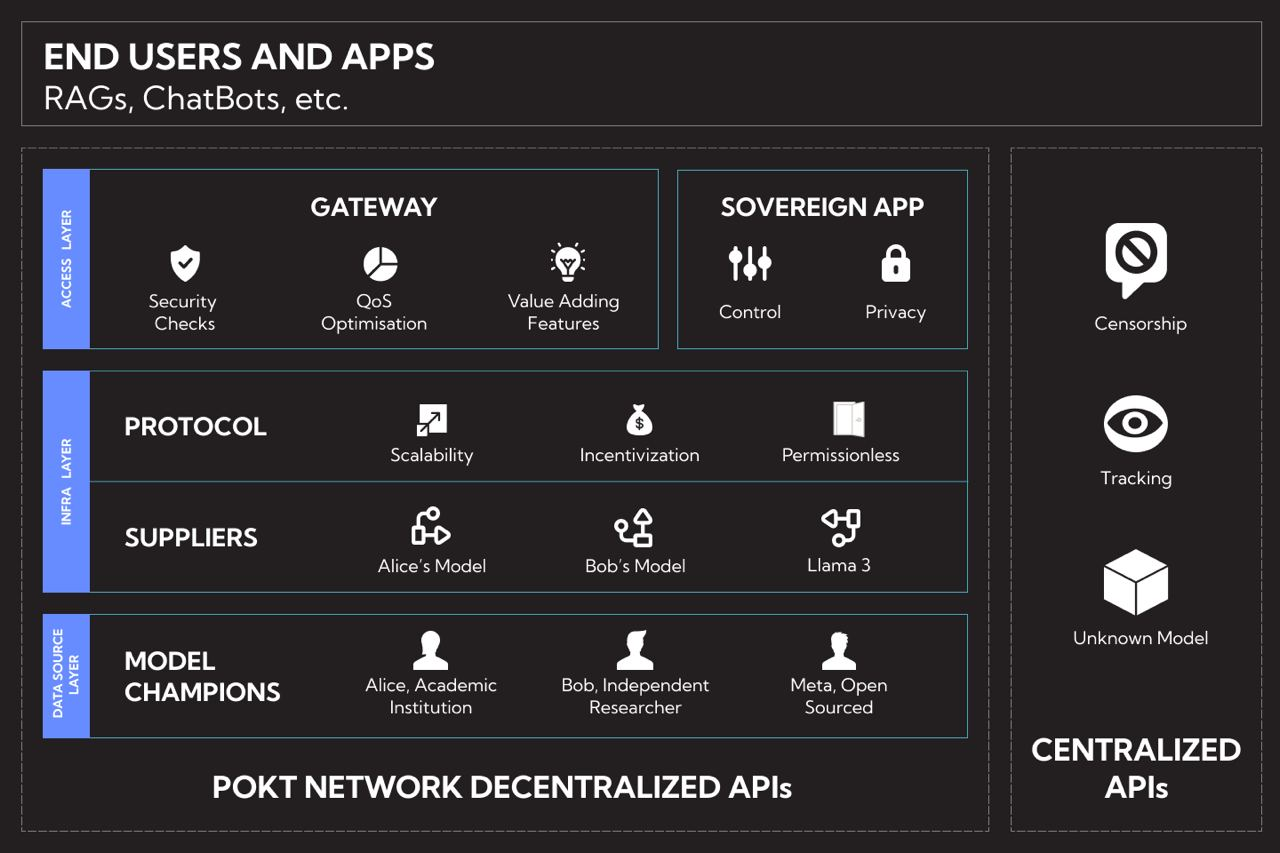
\includegraphics[width=0.9\linewidth]{stakeholders.jpeg}
\caption{Comparison of POKT Network's AI API actors versus centralized API service providers.}
\label{fig_stakeholders}
\end{figure*}


\subsection{Model Providers: Gateways \& Watchers}

Building and maintaining LLM infrastructure is resource intensive and likely to commoditize. As such, model Gateways are poorly incentivized to maintain it themselves, relative to dedicating the same resources to higher value-adding activities.

Gateways provide the product/services layer on top of POKT Network’s decentralized infrastructure. They serve as the entry points between Applications and the POKT Network protocol by facilitating communication and abstracting away the complexity of interacting with the protocol. They play a key part in optimizing the quality of service of the underlying infrastructure (integrity, correctness, reliability, availability, uptime, throughput, latency, security, etc) in order to provide seamless access for AI-enabled applications.

The POKT Network DAO funds and supports an open-source gateway ecosystem~\cite{poktGatewayServer} to make it as easy as possible for anyone with a strong interest in a particular model to build a business selling inference services for that model without having to build any of the underlying infrastructure themselves. The margin opportunity for Gateways comes from providing custom support, including enterprise-level Service Level Agreements (SLAs) \cite{groveSLA}, value-added features and custom pricing. POKT Network’s Gateway ecosystem provides another new and sustainable business model for open-source AI researchers to profit from their work without having to build out a globally scalable infrastructure back-end first.

Watchers are a special type of Gateways that provide checks and guarantees on the underlying Suppliers by discreetly assessing service providers while posing as regular users, ensuring they remain undetected. It offers research communities a valuable tool to assess how models perform in real-world settings, free from any biases or conflicts of interest tied to model creators or users.


\subsection{Model Users: Applications}

Most Applications will likely use Gateways to access the network, but direct access is also possible. This shifts SLA responsibility to the Application itself in exchange for full privacy and sovereignty. For instance, direct access prevents prompts from being aggregated by large Gateways. It also allows Applications to access the model marketplace directly, enabling experimentation with a potentially more diverse set of use cases. Lastly, it should result in cheaper access to services provided by the network as Applications will be able to avoid any off-chain cost structures imposed by the Gateways. 


\subsection{Model Suppliers: Hardware Operators}

Suppliers are entities running inference nodes to earn POKT. They are a crucial social component of any decentralized service network, essential to both bootstrapping and growing, and are one of the most challenging assets to build.

Suppliers' core competencies include DevOps, hardware maintenance, logging, redundancy management, etc. Paired with POKT Network’s economic incentives, these abilities facilitate the rapid adoption of support for inference services across new models.

POKT Network's permissionless approach thrives on minimal friction, allowing Suppliers to stake for any inference model, and encouraging external providers to join the Supplier community. In particular, it creates opportunities to repurpose:

\begin{itemize}
    \item \textbf{Idle Inference Hardware:} Any LLM inference pipeline can be connected to POKT Network with minimal overhead. POKT Network's Relay Mining client is a coprocessor \cite{coprocessor} that acts as a lightweight "sidecar", requiring minimal resources in comparison to the hardware needed for inference.
    \item \textbf{Dormant Calculation Hardware:} Compute servers awaiting large workloads (e.g. model training) can be deployed without long-term leases or commitments. POKT Network provides a secondary revenue stream when models aren't being trained.
    \item \textbf{GPU Mining Hardware for Useful Work:} Proof of Work (PoW) operations can be repurposed to provide tailored inference models. Unlike PoW, electricity is solely used for productive tasks triggered by incoming RPC requests and paid for proportionally to the usage.
\end{itemize}

With a clear task delineation of roles and the right incentives, Suppliers focus on reducing inference costs while maximizing RPC consumption based on user demand. Developing and deploying cost-effective inference strategies, such as model quantization schemes, fast cache handling, and CPU inference, is incentivized and abstracted from the end user.


\subsection{Model Sources: Engineers \& Researchers in AI and ML}
Model Sources are individuals, teams or institutions that open-source newly trained or fine-tuned models. Often seeking users or testers, they lack the capital or expertise to deploy and manage their own performant hardware.

After publishing a model on the network, Sources leverage social forums to drive demand and collaborate with Suppliers to support it. In return, they earn a perennial revenue share from the model's success. This revenue share is a fraction of the fees paid in POKT by Applications to Suppliers for inference services, proportionate to the volume performed (i.e. the number of estimated on-chain requests).

This business model innovation enables researchers at academic institutions to earn revenue from their work's success without building customer-facing infrastructure, making it an attractive opportunity for contributors. Currently, grants and donations are the primary source of revenue supporting such stakeholders~\cite{lmsysDonationsLMSYS}.





\section{Input/Output of a Decentralized Inference Network}

\subsection{LLM Inputs to POKT Network}
The following primitives flow across the stakeholder boundaries outlined earlier. Each is necessary to enable and add value to a decentralized inference network stack.

\begin{itemize}
    \item \textbf{Open-source models:} Models supplied and accessed on the network should be open-source. Proper incentive alignment will drive adoption, solving the issue of altruistic operators common in other open-source ecosystems. Although closed-source models could be provided, this would limit availability to a small set of Suppliers.

    \item \textbf{Inference Demand:} Demand for a particular model must come from end-users or Applications. This demand can arise organically through user discovery, explicitly through model Source owners promoting their models, or via sales brought about by Gateways.

    \item \textbf{Supply Aggregation:} Supply for mid-tier models should come from commodity hardware, not specialized or scarce systems. Aggregating this supply is beneficial when targeting use cases that are too energy-intensive for end-user devices. POKT Network isn't suitable for high-end use cases requiring the latest GPUs, but it democratizes and enables supply and demand for the rest of the market.

    \item \textbf{Quality of Service Guarantees:} Operating on the network must adhere to certain SLAs. Quality can be measured via open-source frameworks, proprietary application logic (e.g., performance metrics), an on-chain reputation system, or a trusted Gateway compensated off-chain.

\end{itemize}

\subsection{LLM Outputs from POKT Network}

Despite the performance and reliability offered by centralized inference providers, they come with tradeoffs in the context of innovation, composability and privacy. For example, centralized services aggregate valuable data for future training, can unilaterally modify model performance, and can censor users at will.

A decentralized solution offers more visibility into the entire stack, benefiting the end-user or Application through the following features:

\begin{itemize}
    \item \textbf{No Downtime:} The probability of AI inference becoming unavailable is much lower since the network is inherently heterogenous, multi-tenant, multi-cloud and decentralized both geographically and geopolitically.

    \item \textbf{Model Experimentation: } Modifying the requested model type is seamless for end users, allowing requests to be routed to many providers using the same underlying protocol.

    \item \textbf{Public Model Evaluation:} Permissionless actors (Gateways, DAOs, Watchers, etc.) can build custom services to verify model performance and Supplier integrity, providing visibility and signal into actor behavior without enforcing specific attributes in the protocol on day one.

    \item \textbf{Privacy Preserving History:} The network operates as a mixing layer, where prompt inputs and inference responses are disseminated across a broader network.
    
    \item \textbf{Censorship-Free Models:}  Being permissionless and decentralized means that models aren’t subject to specific censorship, avoiding the “Woke AI”~\cite{thefpGooglesWoke} issues we’ve seen from large companies.
\end{itemize}

\section{Web3 Ecosystem Integrations}

POKT Network, as the largest decentralized RPC protocol for blockchain data, can integrate with other protocols in the broader Web3 ecosystem to bring additional efficiency and functionality to the Decentralized AI (DecAI) stack. The Pocket Network powers the inference layer of the ecosystem, highlighted in figure~\ref{fig_stack}.


\begin{figure*}[!h]
\centering
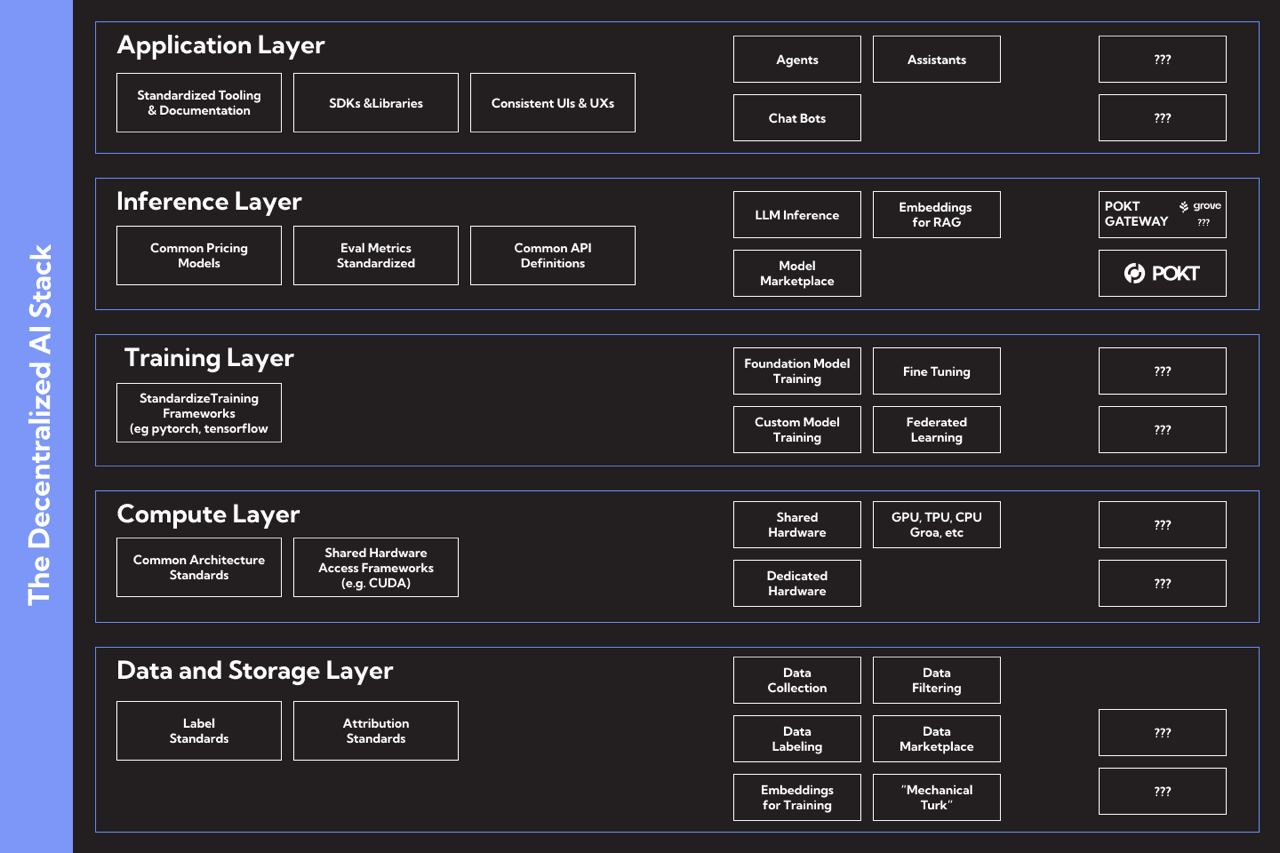
\includegraphics[width=0.9\linewidth]{stack.jpeg}
\caption{Decentralized AI (DecAI) stack showing where POKT Network fits in the Inference Layer.}
\label{fig_stack}
\end{figure*}

\subsection{Data \& Storage Networks}
DecAI inferencing can leverage decentralized storage solutions like Filecoin/IPFS and Arweave, creating seamless integrations between POKT Network Suppliers and other actors in the DecAI stack.

\begin{itemize}
    \item \textbf{Network-Wide Model Storage:} AI models can be easily stored on these networks. It enhances their security, integrity, and immutability while facilitating seamless access and distribution.

    \item \textbf{Verifiable Data Storage:} Decentralized data storage enhances and incentivizes the attribution and sharability of models, labels and potentially even prompts/responses in an immutable manner.

\end{itemize}
For example, a Model owner could train their model offline, upload it to Arweave and simply point a POKT Network Supplier at the pinned file.


\subsection{Compute Networks}
DecAI inferencing can be viewed as a complementary service layer building on top of existing decentralized computing layer solutions. For example, a single POKT Node providing access to Llama 70B could act as a proxy to multiple leased GPU/TPU nodes across Akash, Render, etc to earn additional revenue when it is not used for dedicated training. DecAI inferencing can harness both dedicated or idle hardware, strengthening decentralized compute leasing networks and fostering their growth.

\subsection{Inference Networks}
DecAI inference nodes integrated into POKT Network exhibit versatility as either physical entities or logical constructs. Logical inference nodes provide abstraction and integration capabilities, sourced from diverse components such as coprocessors, agent networks, solver networks, or even inferencing blockchains.

\begin{itemize}
    \item \textbf{Flexible Deployment Model:} This abstraction enables flexible deployment and seamless integration with various DecAI infrastructural elements, accommodating different computational architectures and workflows.

    \item \textbf{Robust Ecosystem:} Physical or logical DecAI nodes contribute to a robust ecosystem supporting a wide range of inference tasks, fostering innovation and efficiency.

\end{itemize}

\subsection{Applications}
DecAI inferencing enables diverse applications, ranging from AI agents and assistants, to consumer apps and Gateways.
\begin{itemize}
    \item \textbf{AI Agents \& Assistants:} These leverage DecAI inference for personalized recommendations, task automation, and natural language understanding to enhance user experiences.

    \item \textbf{Consumer Apps:} Benefit from DecAI inference by delivering tailored content, optimizing interactions, and safeguarding data privacy.

    \item \textbf{Gateways \& IoT:} Analyze sensor data, detect anomalies, and enable autonomous edge decision-making.
\end{itemize}

\section{Conclusion}
By leveraging its established infrastructure, verifiable guarantees, and crypto-economic design, POKT Network unlocks a new infrastructure stack for open-source AI. Building on top of an ecosystem of Suppliers and Gateways that have been facilitating hundreds of millions of daily blockchain RPC requests, LLM inference stands to gain from the same reliable, performant and cost-effective services offered by the network.

POKT Network creates a utility providing bridge between open-source AI and Web3 to create new revenue streams for AI researchers without needing to maintain infrastructure or user-facing applications. In particular, AI researchers can now directly benefit from demand for their work without having to restrict access or needing to raise large amounts of capital to monetise it. While doing so, the network can leverage mid-tier idle compute resources that do not need to be exclusively leased in use-cases such as training. 

This enables POKT's stakeholders (Sources, Applications, Suppliers, and Gateways) to build innovative, sustainable, reliable, and verifiable services. Taken together, POKT Network’s approach enables a greater diversity of models to experiment with, better market access to inference infrastructure for small and medium-sized enterprises and a new sustainable business model for open-source AI researchers.

With POKT Network’s ecosystem-led approach to providing inference services, on-chain and off-chain innovation can move in parallel without being overly constrained by one another. Additionally, there are significant opportunities for integration across Web3 protocols, building the foundation for a standardized Decentralized AI stack.

This paper outlined a realistic and tangible vision that POKT Network can bring to the ecosystem in the near future. Further research and development will continue to expand the ecosystem's potential and scope, ensuring that the POKT Network remains a robust and adaptable solution within the swiftly evolving AI and blockchain landscapes.

\section{Future Work}
The intersection of POKT and AI is a broad subject, and many engaging and critical topics remain as future work. The following is a non-exhaustive list summarizing key areas of active research and development.

\begin{itemize}
    \item \textbf{Tokenomics:} Centralized services may offer superior short-term performance, but decentralized networks can accrue and provide more value as they expand. Rapid iterations in LLMs require a comprehensive tokenomics document aligning incentives with common LLM inference performance metrics~\cite{databricksInferencePerformance} like input/output token counts, Time To First Token (TTFT), Time Per Output Token (TPOT), Latency, Throughput, etc.

    \item \textbf{Trusted Execution Environment (TEE):} POKT Network can offer TEE as a marketplace option, letting users choose whether inference should be executed in a TEE. Suppliers can offer TEE via Intel SGX~\cite{intelIntelSoftware}, AMD SEV~\cite{amdsev}, AWS Nitro~\cite{amazonLightweightHypervisor}, ARM TrustZone~\cite{armTrustZoneCortexA}, etc., saving users operational overhead and earning additional revenue.

    \item \textbf{Model inference verification:} Verifying the quality and origin of model outputs is a still an active area of research, especially in a permissionless network. Our approach aims to enhance, not limit, model diversity, which introduces a new set of challenges. For example, a Supplier advertising Llama:70B may be running speculative decoding~\cite{leviathan2023fast} or even a Llama:7B to cut costs. Similar to how new strategies were developed and adopted to tackle permissionless quality-of-service as blockchain RPC volume grew, we anticipate new solutions to emerge as the network traffic for LLMs grows as well. A non-exhaustive list of approaches under active R\&D include Suppliers operating on Trusted Execution Environments (TEEs), probabilistic non-interactive on-chain quorum checks, public evaluation benchmarks by Gateways, watermarked on-chain models \cite{watermarking} or somewhat homomorphic encryption of private models \cite{cryptoeprint:2013/422}. Initially, we also anticipate "vibe based development" by Applications \cite{simonWillisonVibes} to re-route traffic to more performant actors or provide the necessary signal for Gateways that certain Suppliers may be faulty, low-quality or adversarial.
    
    \item \textbf{Adversarial Play:} Closely related to the game theory connecting tokenomics to model verification, attack mitigation requires its own dedicated document. In a permissionless environment, bad actors staking low-quality models are expected. Addressing this challenge is integral to the protocol. A separate document will be published dedicated to this topic, iterating on the tokenomics that have been driving POKT Network's sustainability over the last three plus years.


\end{itemize}

The work outlined above is a starting point and foundation layer for POKT Network's journey into DecAI. This list doesn't constrain the protocol's future, as POKT Network will continue exploring opportunities and refining the roadmap.













% An example of a floating figure using the graphicx package.
% Note that \label must occur AFTER (or within) \caption.
% For figures, \caption should occur after the \includegraphics.
% Note that IEEEtran v1.7 and later has special internal code that
% is designed to preserve the operation of \label within \caption
% even when the captionsoff option is in effect. However, because
% of issues like this, it may be the safest practice to put all your
% \label just after \caption rather than within \caption{}.
%
% Reminder: the "draftcls" or "draftclsnofoot", not "draft", class
% option should be used if it is desired that the figures are to be
% displayed while in draft mode.
%
%\begin{figure}[!t]
%\centering
%\includegraphics[width=2.5in]{myfigure}
% where an .eps filename suffix will be assumed under latex, 
% and a .pdf suffix will be assumed for pdflatex; or what has been declared
% via \DeclareGraphicsExtensions.
%\caption{Simulation results for the network.}
%\label{fig_sim}
%\end{figure}

% Note that the IEEE typically puts floats only at the top, even when this
% results in a large percentage of a column being occupied by floats.


% An example of a double column floating figure using two subfigures.
% (The subfig.sty package must be loaded for this to work.)
% The subfigure \label commands are set within each subfloat command,
% and the \label for the overall figure must come after \caption.
% \hfil is used as a separator to get equal spacing.
% Watch out that the combined width of all the subfigures on a 
% line do not exceed the text width or a line break will occur.
%
%\begin{figure*}[!t]
%\centering
%\subfloat[Case I]{\includegraphics[width=2.5in]{box}%
%\label{fig_first_case}}
%\hfil
%\subfloat[Case II]{\includegraphics[width=2.5in]{box}%
%\label{fig_second_case}}
%\caption{Simulation results for the network.}
%\label{fig_sim}
%\end{figure*}
%
% Note that often IEEE papers with subfigures do not employ subfigure
% captions (using the optional argument to \subfloat[]), but instead will
% reference/describe all of them (a), (b), etc., within the main caption.
% Be aware that for subfig.sty to generate the (a), (b), etc., subfigure
% labels, the optional argument to \subfloat must be present. If a
% subcaption is not desired, just leave its contents blank,
% e.g., \subfloat[].


% An example of a floating table. Note that, for IEEE style tables, the
% \caption command should come BEFORE the table and, given that table
% captions serve much like titles, are usually capitalized except for words
% such as a, an, and, as, at, but, by, for, in, nor, of, on, or, the, to
% and up, which are usually not capitalized unless they are the first or
% last word of the caption. Table text will default to \footnotesize as
% the IEEE normally uses this smaller font for tables.
% The \label must come after \caption as always.
%
%\begin{table}[!t]
%% increase table row spacing, adjust to taste
%\renewcommand{\arraystretch}{1.3}
% if using array.sty, it might be a good idea to tweak the value of
% \extrarowheight as needed to properly center the text within the cells
%\caption{An Example of a Table}
%\label{table_example}
%\centering
%% Some packages, such as MDW tools, offer better commands for making tables
%% than the plain LaTeX2e tabular which is used here.
%\begin{tabular}{|c||c|}
%\hline
%One & Two\\
%\hline
%Three & Four\\
%\hline
%\end{tabular}
%\end{table}


% Note that the IEEE does not put floats in the very first column
% - or typically anywhere on the first page for that matter. Also,
% in-text middle ("here") positioning is typically not used, but it
% is allowed and encouraged for Computer Society conferences (but
% not Computer Society journals). Most IEEE journals/conferences use
% top floats exclusively. 
% Note that, LaTeX2e, unlike IEEE journals/conferences, places
% footnotes above bottom floats. This can be corrected via the
% \fnbelowfloat command of the stfloats package.






% conference papers do not normally have an appendix



% use section* for acknowledgment
\ifCLASSOPTIONcompsoc
  % The Computer Society usually uses the plural form
  \section*{Acknowledgments}
\else
  % regular IEEE prefers the singular form
  \section*{Acknowledgment}
\fi


The authors would like to thank Adrienne and Dermot from the POKT Network Foundation for their guidance and graphics construction and the whole POKT Network community for the feedback that helped to shape this document.





% trigger a \newpage just before the given reference
% number - used to balance the columns on the last page
% adjust value as needed - may need to be readjusted if
% the document is modified later
%\IEEEtriggeratref{8}
% The "triggered" command can be changed if desired:
%\IEEEtriggercmd{\enlargethispage{-5in}}

% references section

% can use a bibliography generated by BibTeX as a .bbl file
% BibTeX documentation can be easily obtained at:
% http://mirror.ctan.org/biblio/bibtex/contrib/doc/
% The IEEEtran BibTeX style support page is at:
% http://www.michaelshell.org/tex/ieeetran/bibtex/
\bibliographystyle{IEEEtran}
% argument is your BibTeX string definitions and bibliography database(s)
\bibliography{refs}
%
% <OR> manually copy in the resultant .bbl file
% set second argument of \begin to the number of references
% (used to reserve space for the reference number labels box)
% \begin{thebibliography}{1}

% \bibitem{IEEEhowto:kopka}
% H.~Kopka and P.~W. Daly, \emph{A Guide to \LaTeX}, 3rd~ed.\hskip 1em plus
%   0.5em minus 0.4em\relax Harlow, England: Addison-Wesley, 1999.

% \end{thebibliography}




% that's all folks
\end{document}


